\PassOptionsToPackage{unicode=true}{hyperref} % options for packages loaded elsewhere
\PassOptionsToPackage{hyphens}{url}
%
\documentclass[]{article}
\usepackage{lmodern}
\usepackage{amssymb,amsmath}
\usepackage{ifxetex,ifluatex}
\usepackage{fixltx2e} % provides \textsubscript
\ifnum 0\ifxetex 1\fi\ifluatex 1\fi=0 % if pdftex
  \usepackage[T1]{fontenc}
  \usepackage[utf8]{inputenc}
  \usepackage{textcomp} % provides euro and other symbols
\else % if luatex or xelatex
  \usepackage{unicode-math}
  \defaultfontfeatures{Ligatures=TeX,Scale=MatchLowercase}
\fi
% use upquote if available, for straight quotes in verbatim environments
\IfFileExists{upquote.sty}{\usepackage{upquote}}{}
% use microtype if available
\IfFileExists{microtype.sty}{%
\usepackage[]{microtype}
\UseMicrotypeSet[protrusion]{basicmath} % disable protrusion for tt fonts
}{}
\IfFileExists{parskip.sty}{%
\usepackage{parskip}
}{% else
\setlength{\parindent}{0pt}
\setlength{\parskip}{6pt plus 2pt minus 1pt}
}
\usepackage{hyperref}
\hypersetup{
            pdfborder={0 0 0},
            breaklinks=true}
\urlstyle{same}  % don't use monospace font for urls
\setlength{\emergencystretch}{3em}  % prevent overfull lines
\providecommand{\tightlist}{%
  \setlength{\itemsep}{0pt}\setlength{\parskip}{0pt}}
\setcounter{secnumdepth}{0}
% Redefines (sub)paragraphs to behave more like sections
\ifx\paragraph\undefined\else
\let\oldparagraph\paragraph
\renewcommand{\paragraph}[1]{\oldparagraph{#1}\mbox{}}
\fi
\ifx\subparagraph\undefined\else
\let\oldsubparagraph\subparagraph
\renewcommand{\subparagraph}[1]{\oldsubparagraph{#1}\mbox{}}
\fi

\usepackage{graphicx}
\usepackage[left=2cm,right=2cm]{geometry}

% set default figure placement to htbp
\makeatletter
\def\fps@figure{htbp}
\makeatother

\newcommand{\mbf}{\mathbf}

\usepackage{float}

\begin{document}

\title{Neuro 120 HW3}
\author{Sam Lurye, Gerardo Parra}
\date{October 18, 2018}
\maketitle

\section*{Problem 1}
\subsection*{1a}
\begin{figure}[H]
    \centering
    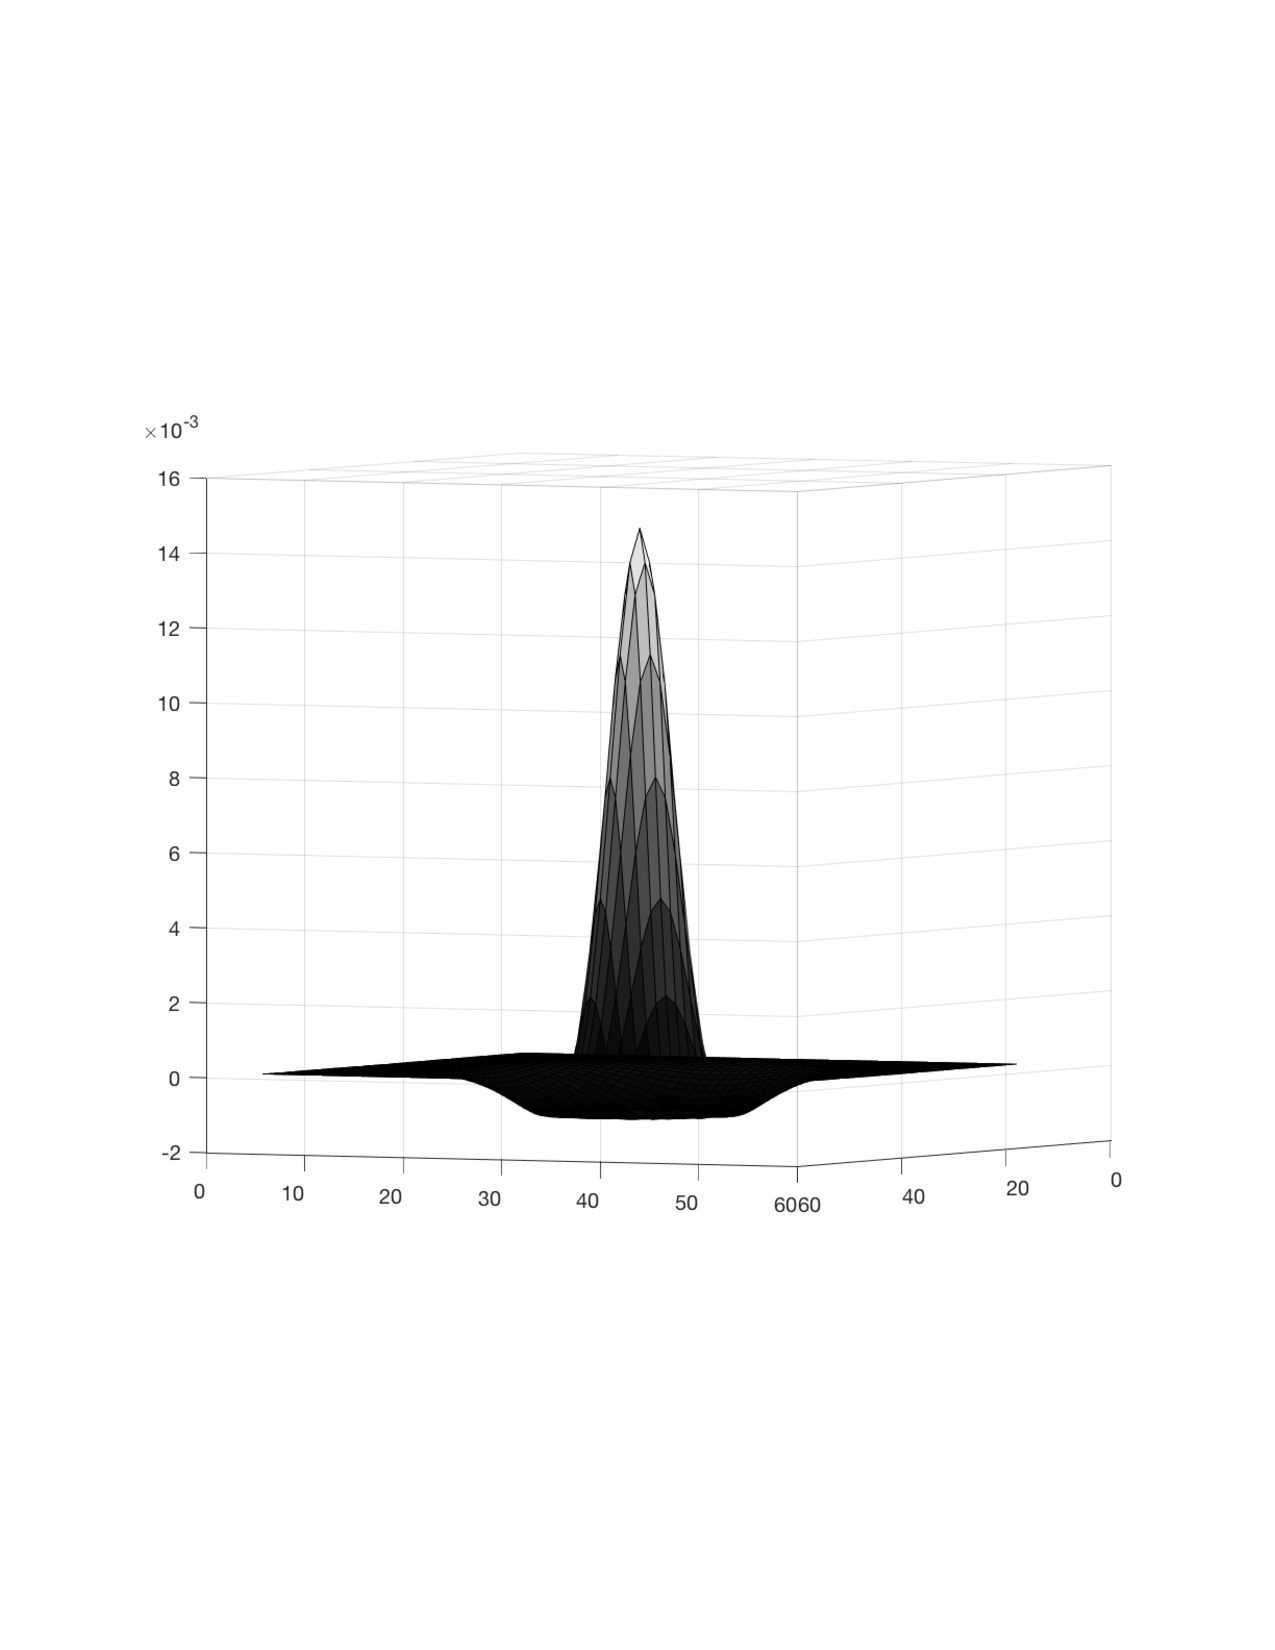
\includegraphics[width=0.7\linewidth]{problem1A.pdf}
    \label{fig:my_label}
\end{figure}

\subsection*{1b}
\begin{figure}[H]
    \centering
    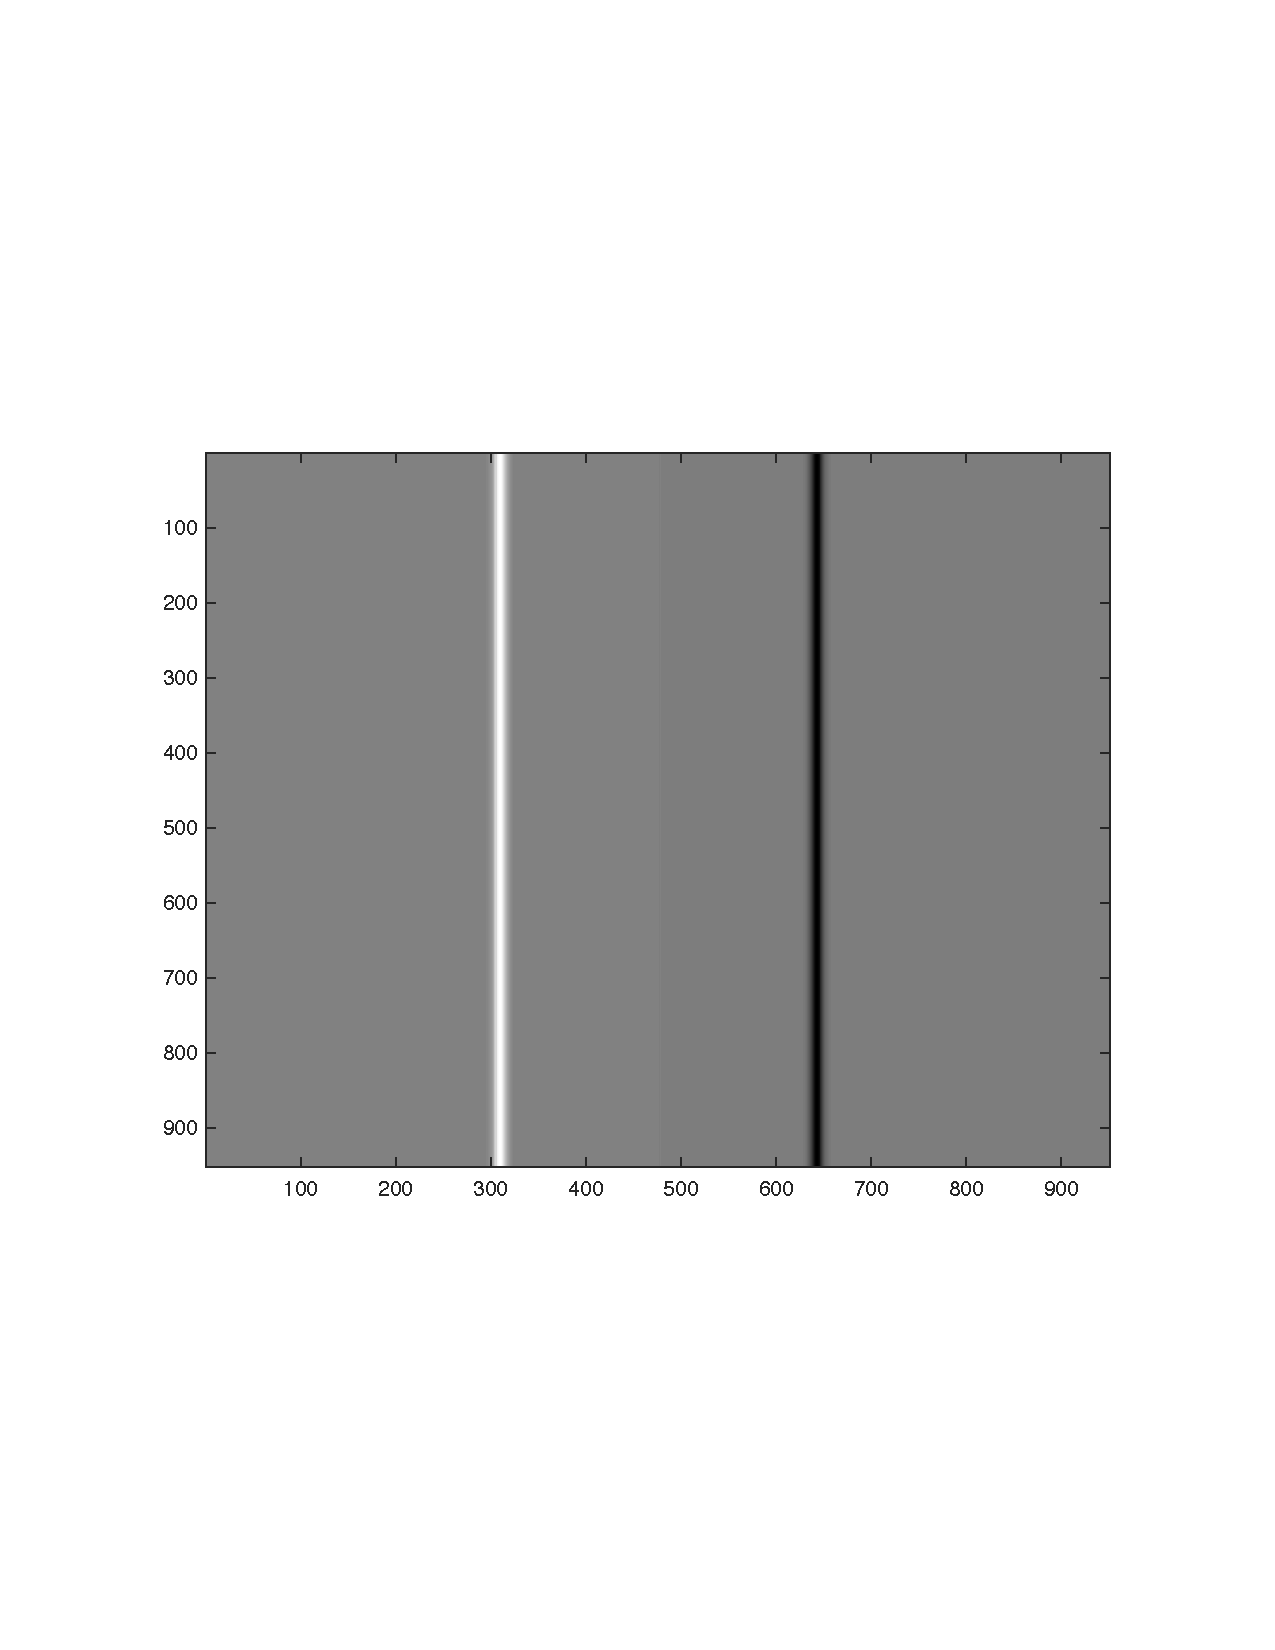
\includegraphics[width=0.7\linewidth]{problem1B.pdf}
    \caption{Assuming that the true RGC response is well approximated by a DoG filter, then we can see that there are two distinct bands in the image in which the RGC response is markedly higher and markedly lower, respectively, than in the rest of the image. This would explain why in the illusion, we perceive two bands that aren't really there in the locations corresponding to these incongruous RGC responses.}
    \label{fig:my_label}
\end{figure}

\subsection*{1c}
\begin{figure}[H]
    \centering
    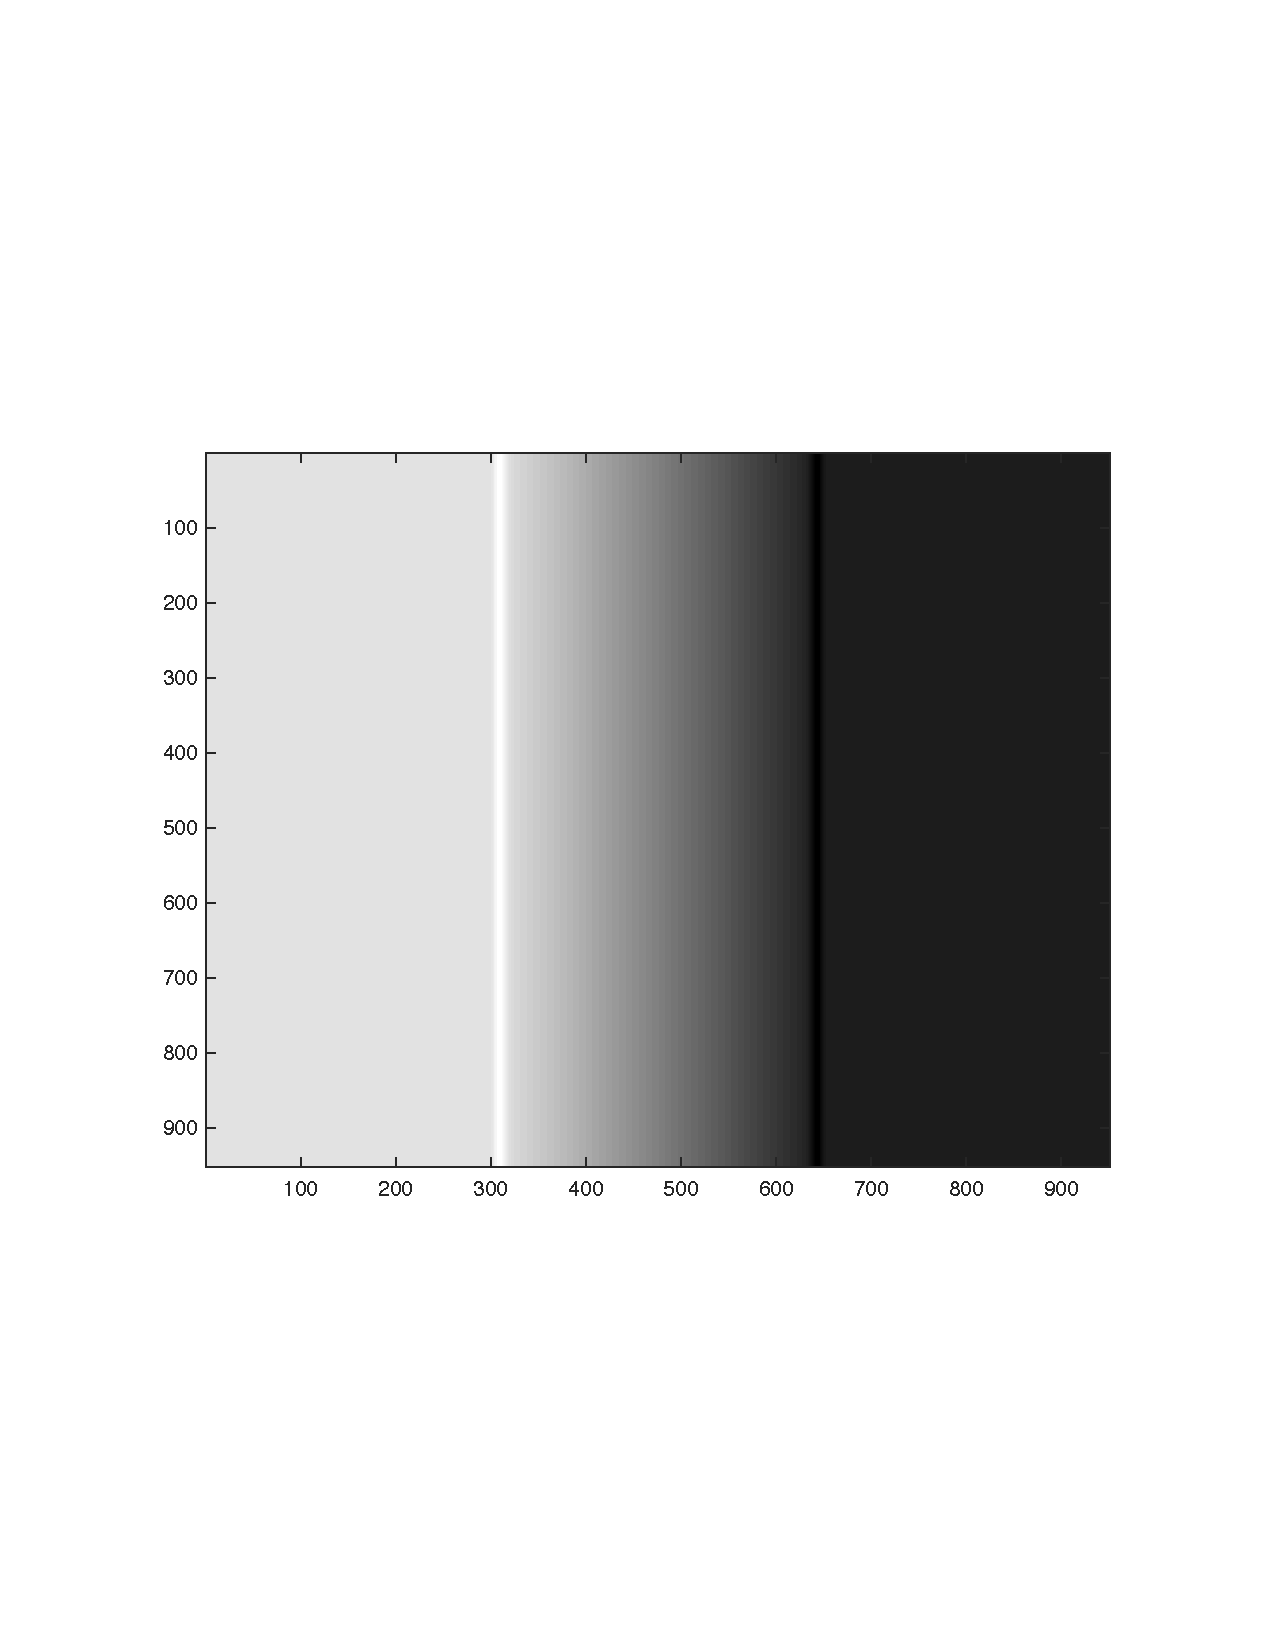
\includegraphics[width=0.7\linewidth]{problem1C.pdf}
    \caption{This result mostly gives us the same information as in 1b. However, it also tells us that the amplified and diminished bands of RGC responses persist even when the RGCs are sensitive to luminance.}
    \label{fig:my_label}
\end{figure}

\subsection*{1d}
\begin{figure}[H]
    \centering
    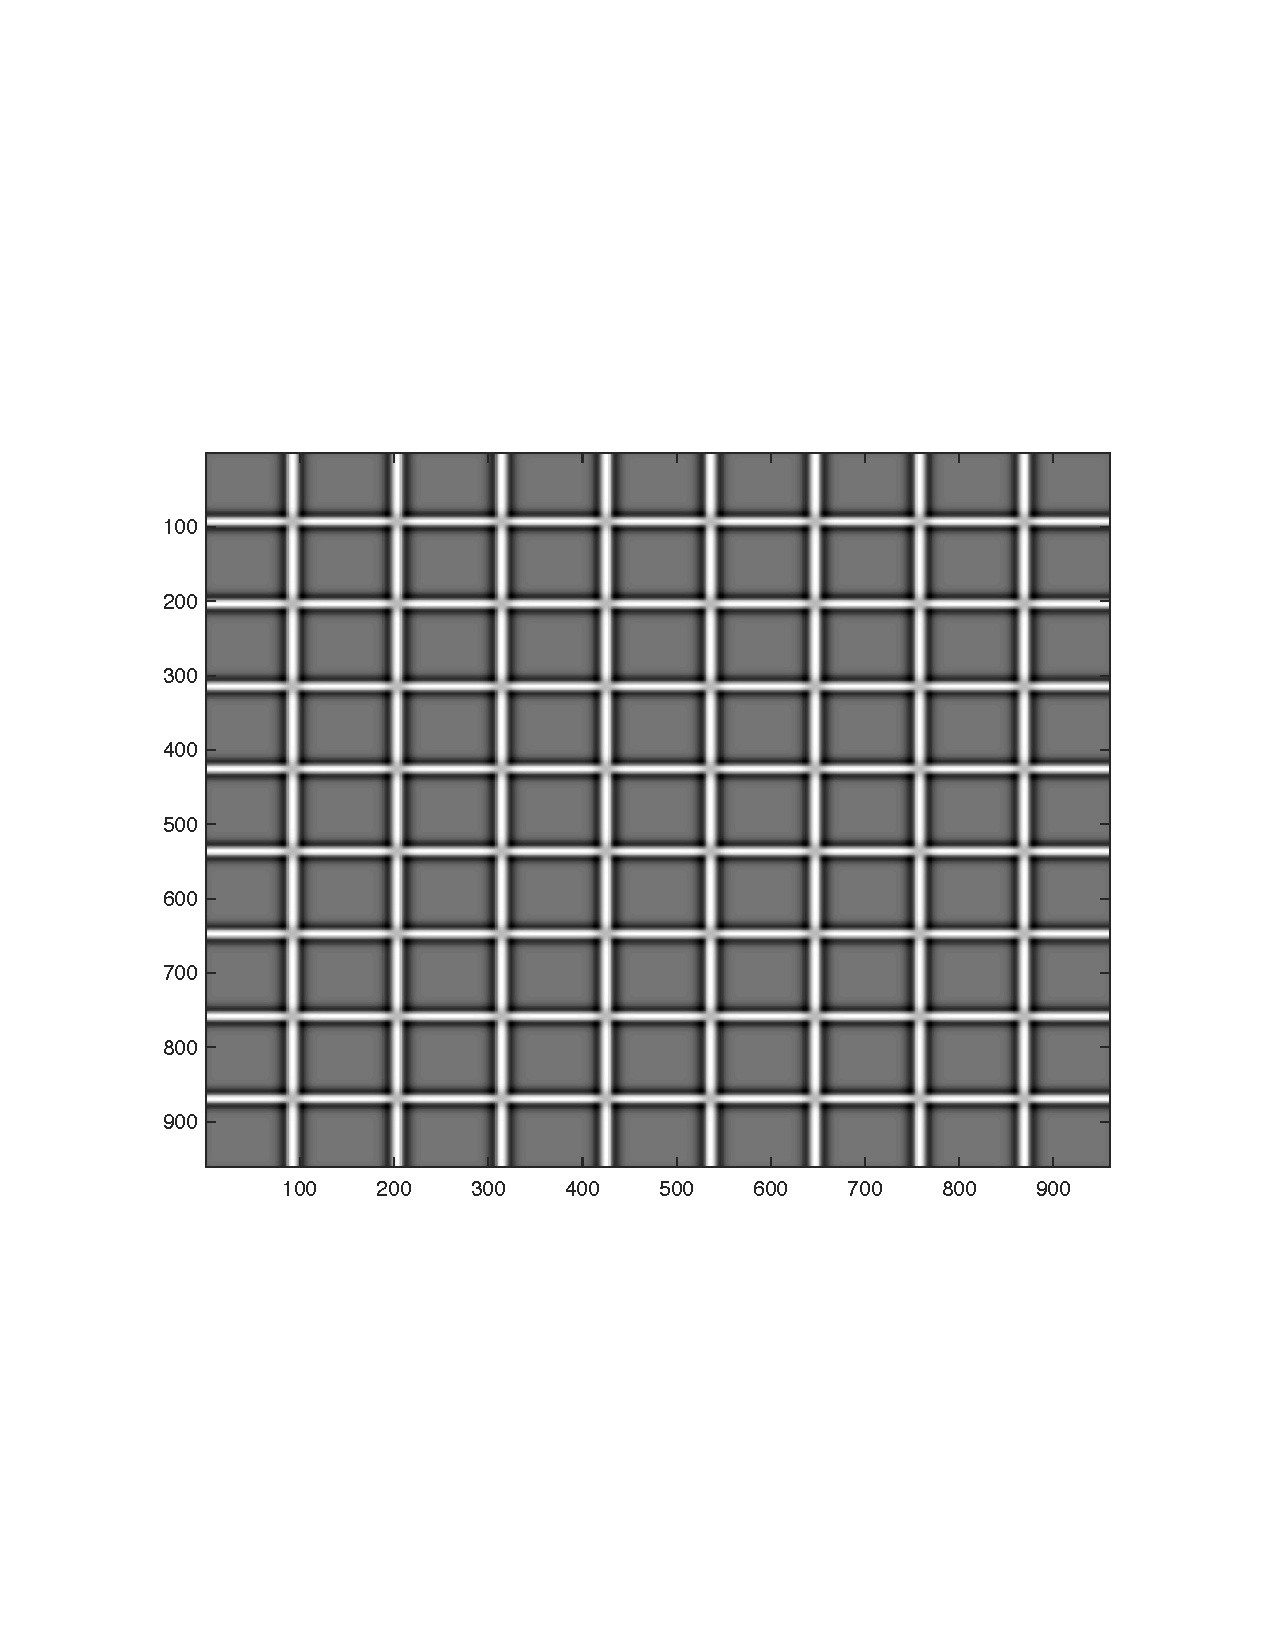
\includegraphics{problem1D.pdf}
    \caption{By zooming in closely, we can see that the RGC response at the intersections of the stripes is less than the response in the middle of a stripe between intersections. This would directly explain why we perceive the intersections to be darker relative to the true color of the stripes.}
    \label{fig:my_label}
\end{figure}

\subsection*{1e}
\begin{figure}[H]
    \centering
    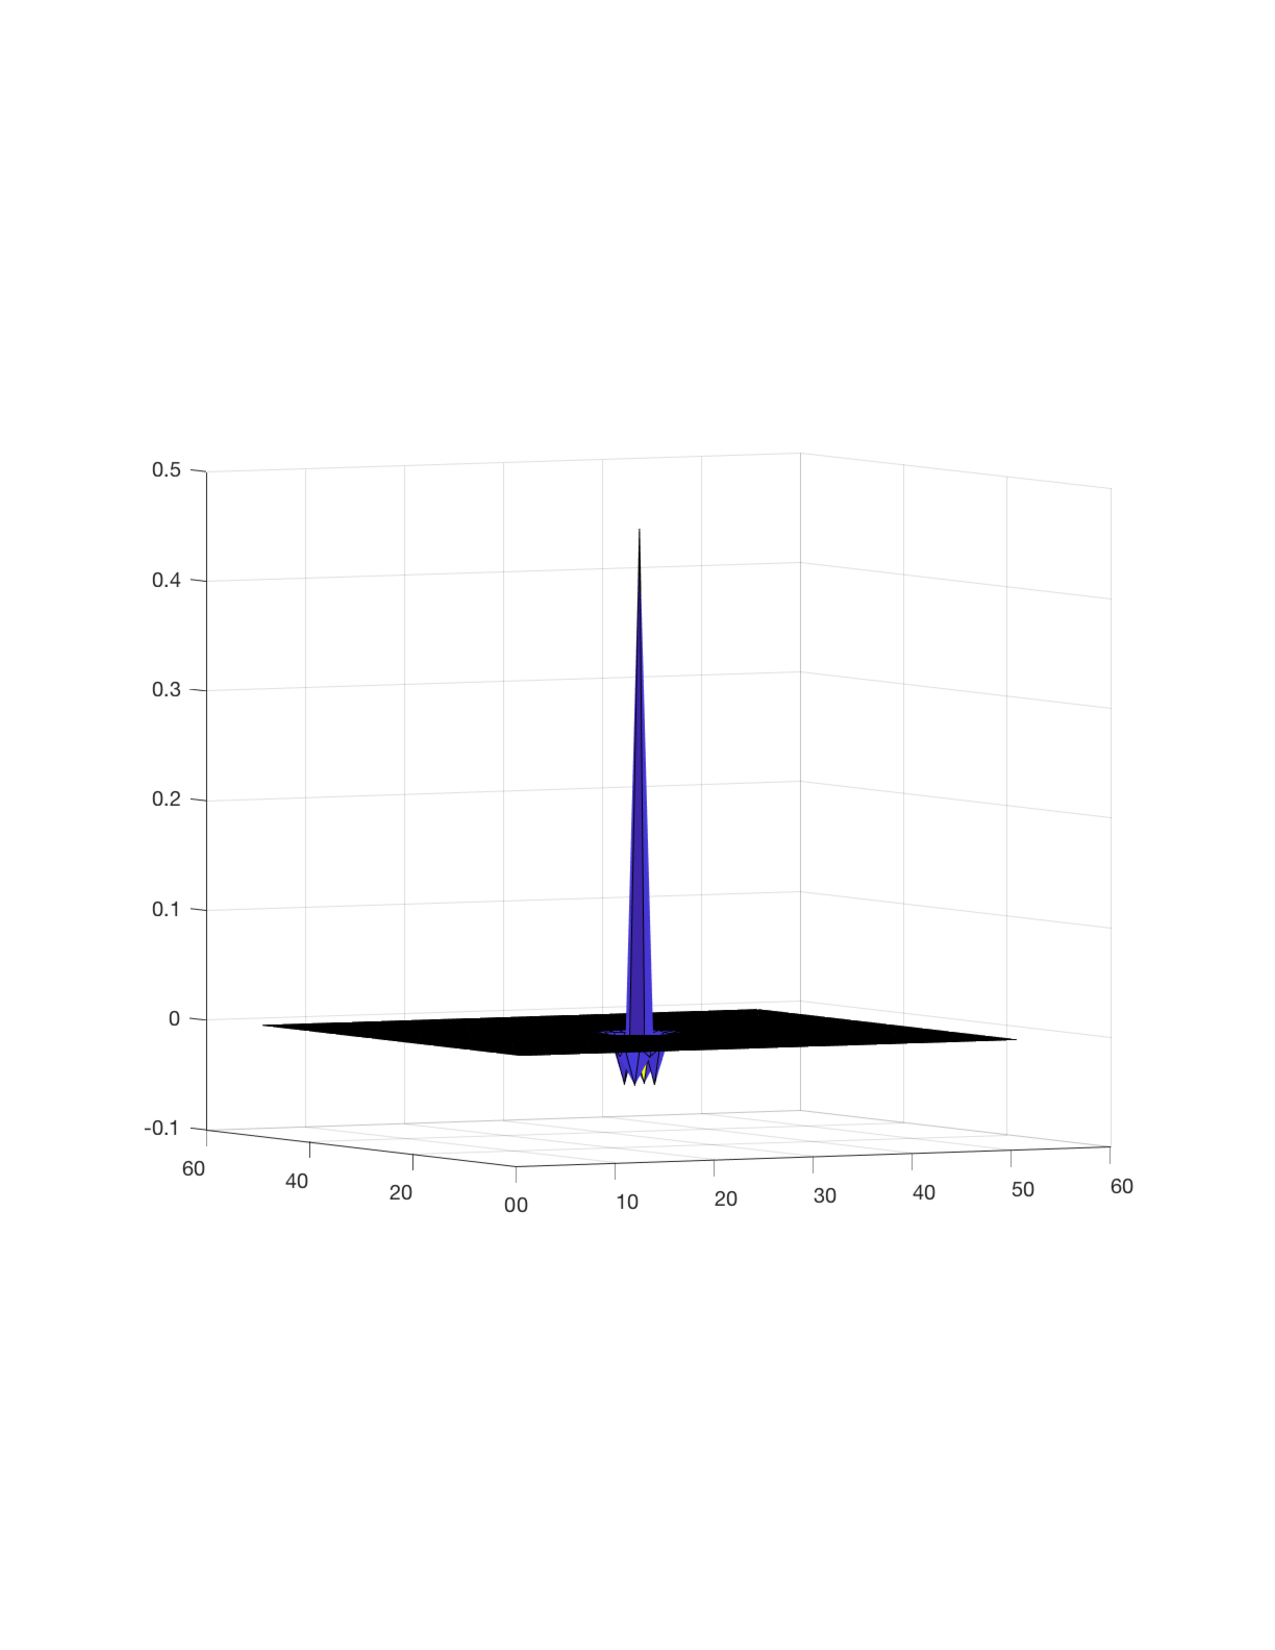
\includegraphics{problem1Esurf.pdf}
    \label{fig:my_label}
\end{figure}
\begin{figure}[H]
    \centering
    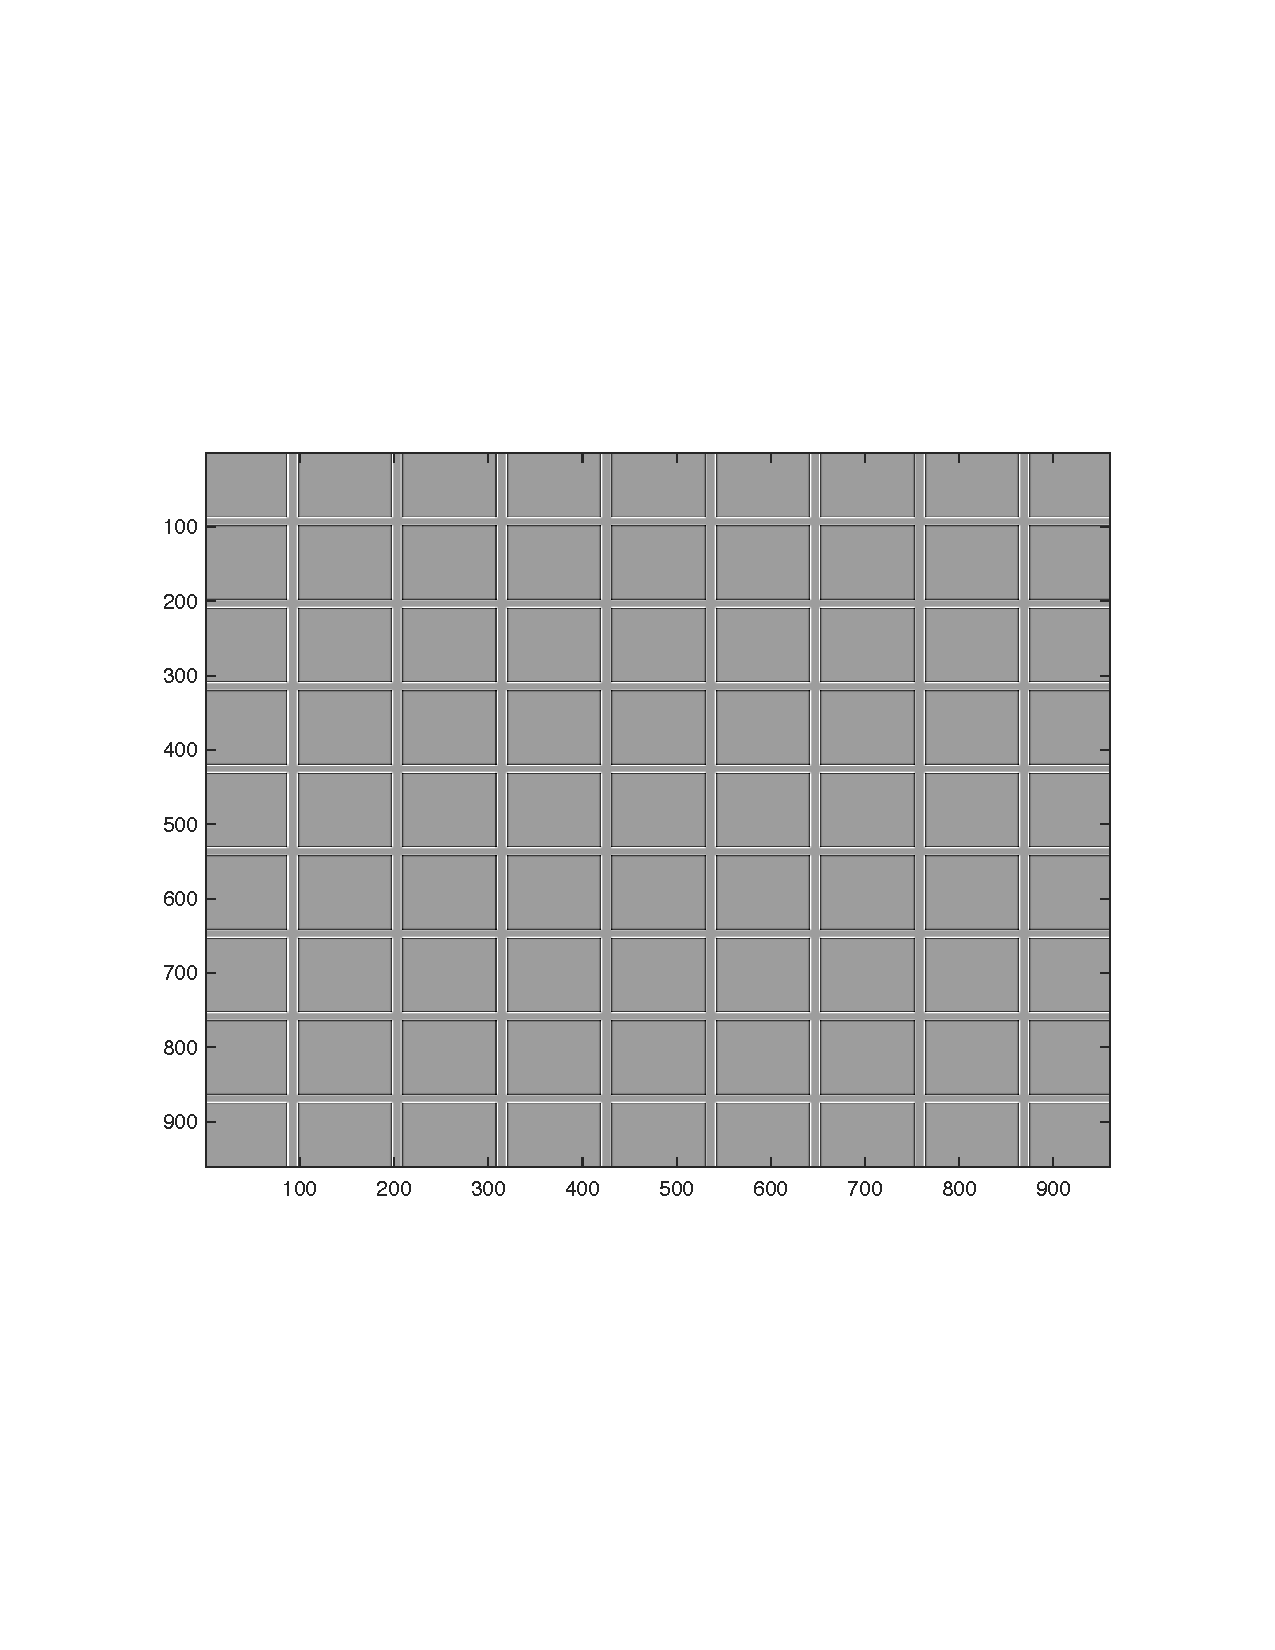
\includegraphics{problem1E.pdf}
    \caption{Unlike in 1d, the RGC response here at the intersections of the stripes is essentially the same as the RGC response elsewhere in the stripes. This explains why in central vision, the stripes appear to be a mostly uniform color, while in peripheral vision there appear to be dark spots at the intersections.}
    \label{fig:my_label}
\end{figure}

\subsection*{1f}
\begin{figure}[H]
    \centering
    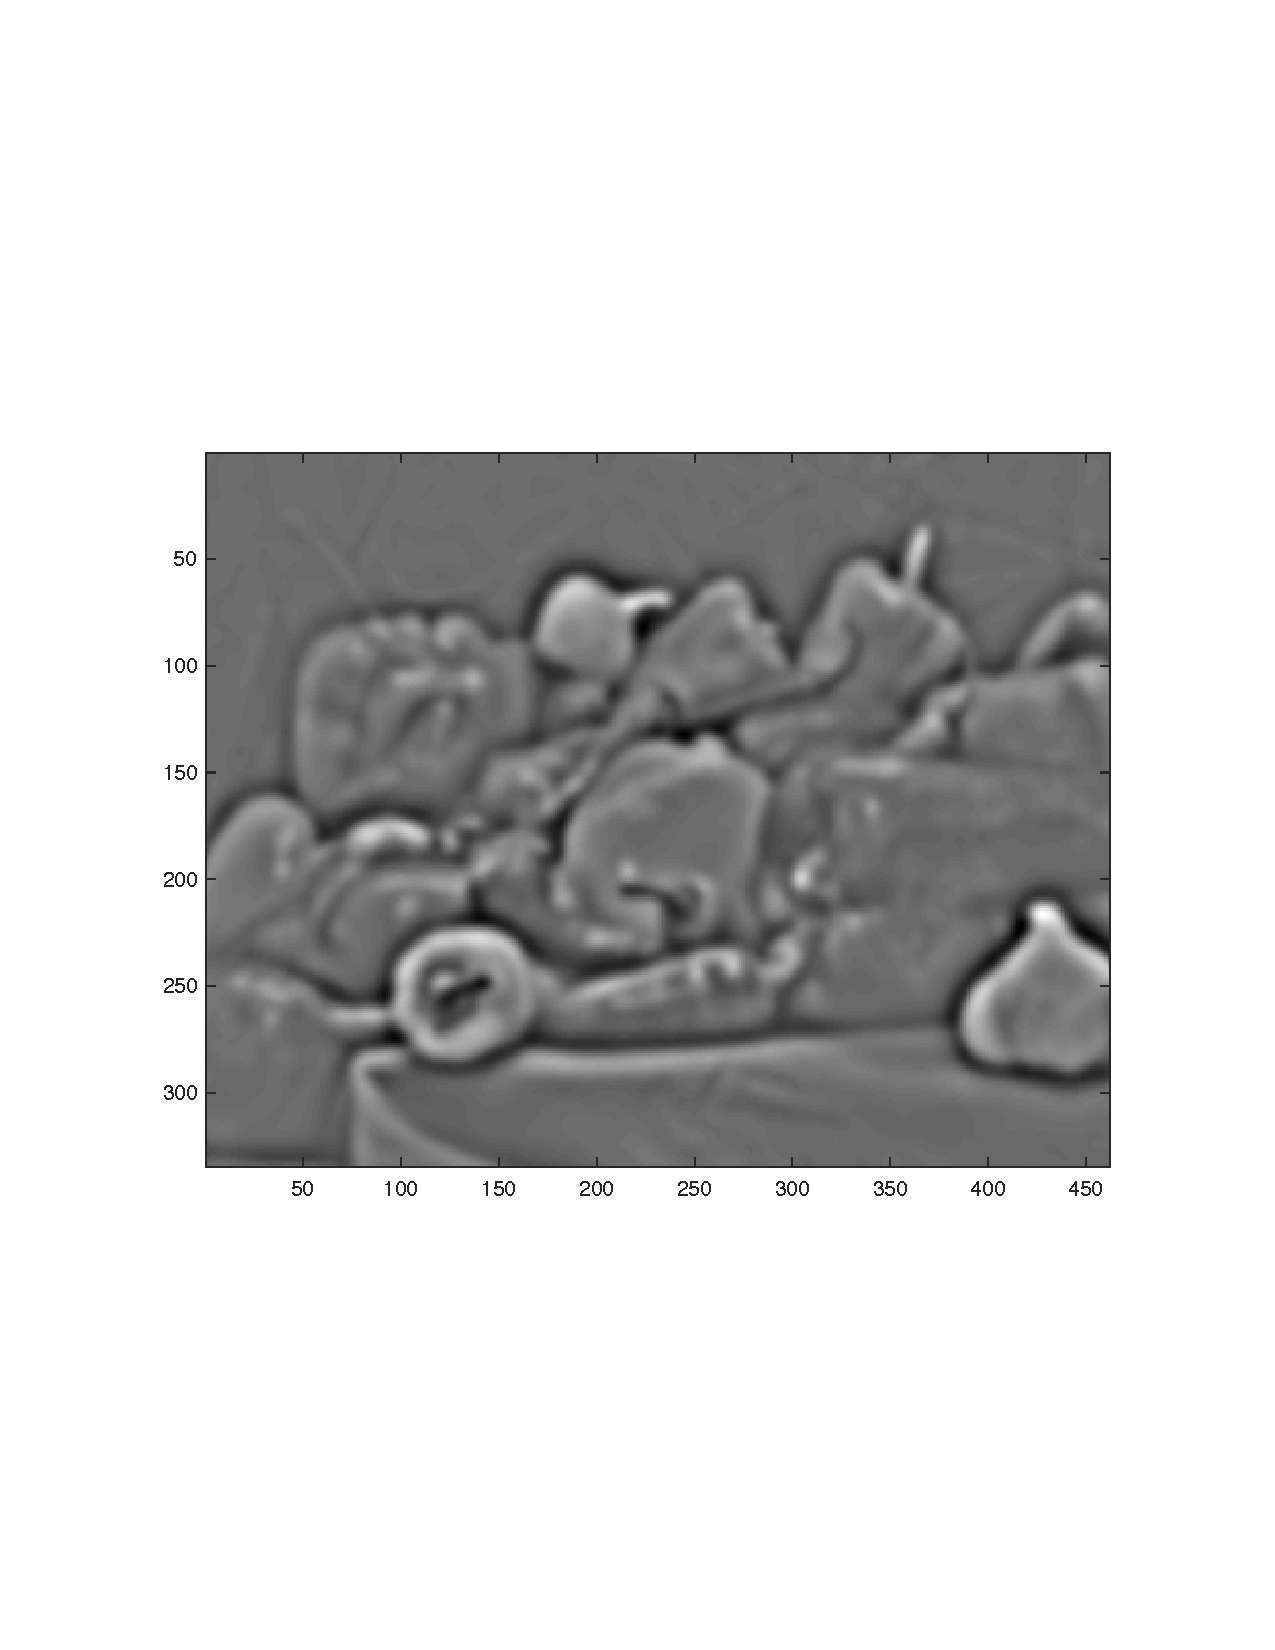
\includegraphics{problem1FfilterA.pdf}
    \caption{Natural image convolved with the filter from part A.}
    \label{fig:my_label}
\end{figure}
\begin{figure}[H]
    \centering
    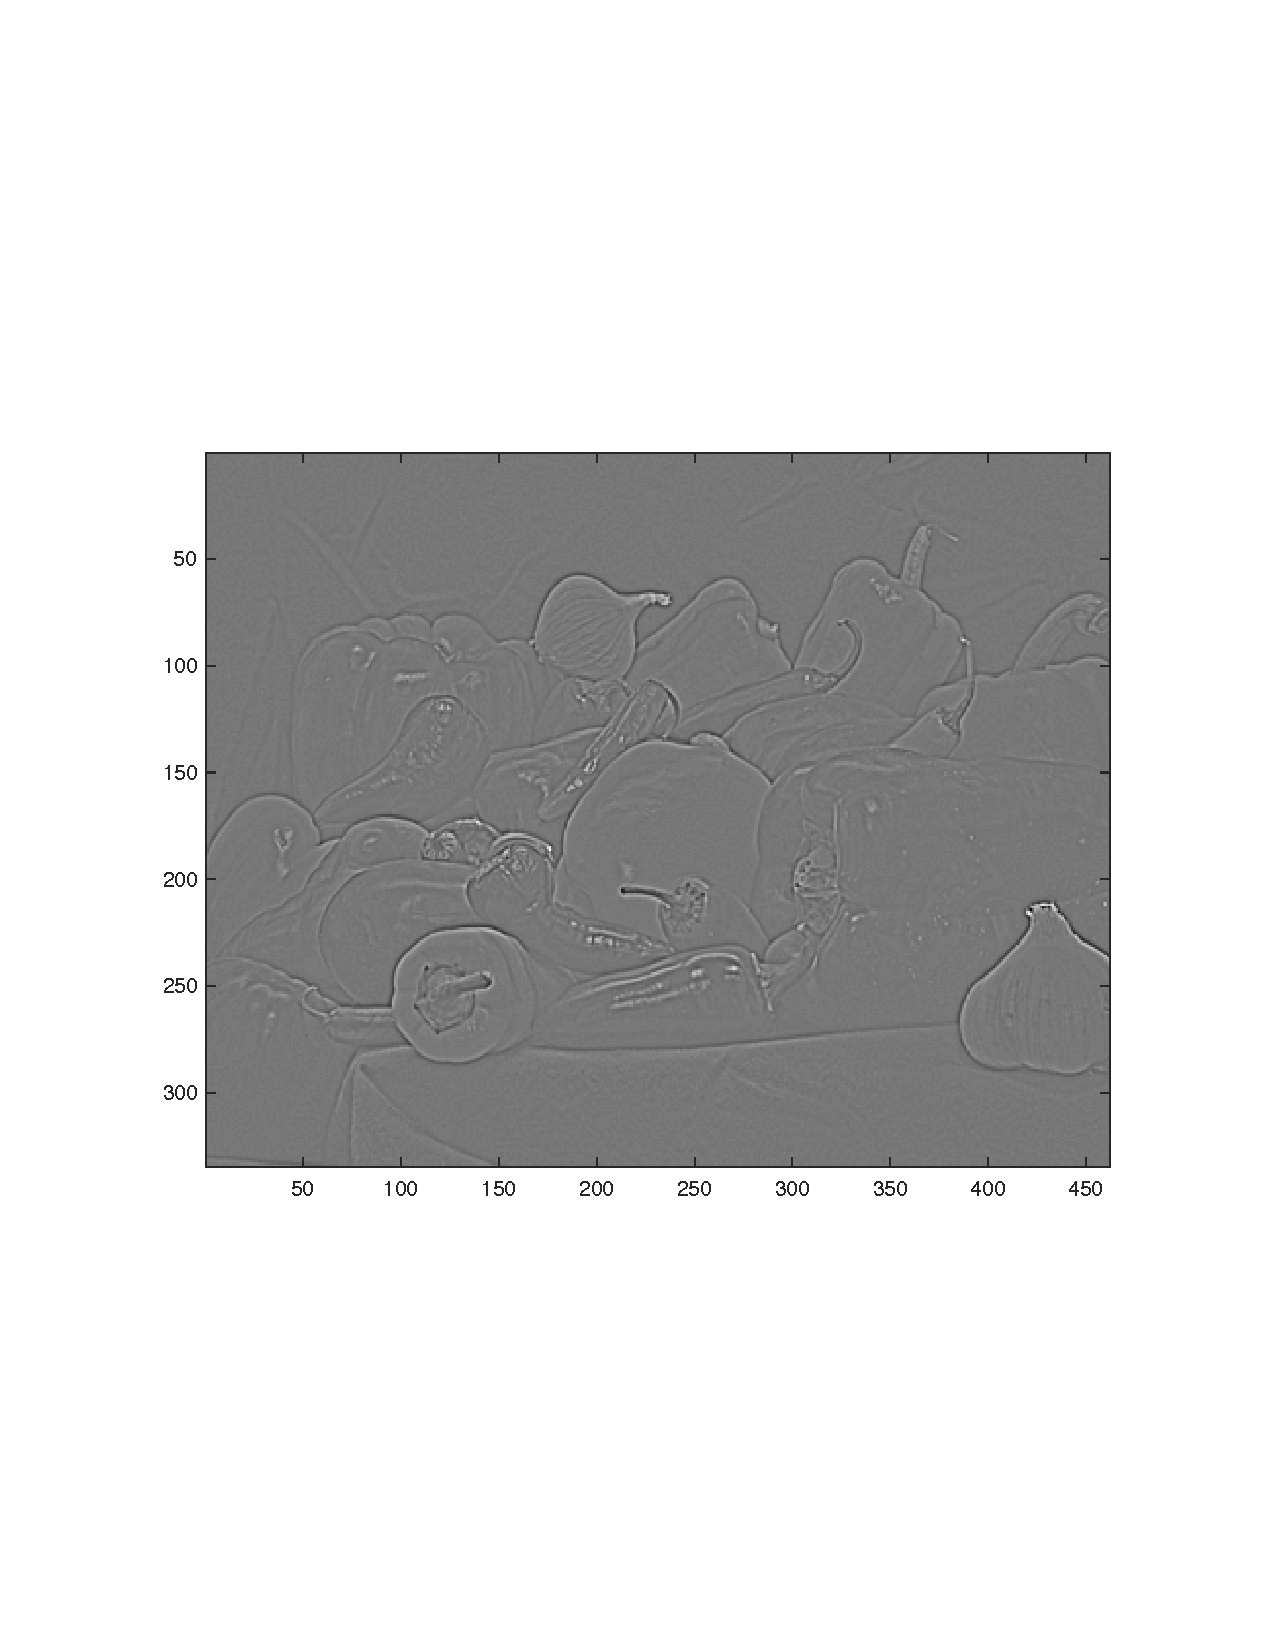
\includegraphics{problem1FfilterE.pdf}
    \caption{Natural image convolved with the filter from part E.}
    \label{fig:my_label}
\end{figure}

The filter from part A, unsurprisingly, produces a much blurrier image than the filter from part E, which makes sense given the higher standard deviation in the filter from part A. Both filters are sensitive to edges and areas of high contrast in the image. However, the filter from part E more precisely outlines objects and preserves fine edge detail, while the filter from part E just gives a more general sense of where the areas of very high contrast are, as we can see in the thick black outlines around, for example, the object in the bottom right corner.

\section*{Problem 2}
\subsection*{2a}
\begin{figure}[H]
    \centering
    \includegraphics[width=0.7\linewidth]{problem2A.pdf}
    \caption{Primarily, the filters are sensitive to oriented edges. The filters in which there are more stripes most closely resemble complex cells, in that they will respond to edges in a way that is more invariant to the position of the edge in their receptive field. Alternatively, the filters with fewer, thicker stripes are more like simple cells, in that the edge must be at a specific position in the receptive field to produce a response. We can also see several center-surround-like filters, which would function similarly to RGCs. Additionally, some neurons appear to respond only to relative luminance (grayscale), while other neurons respond to specific colors.}
    \label{fig:my_label}
\end{figure}

\subsection*{2b}
The network does correctly classify the image.
\begin{figure}[H]
    \centering
    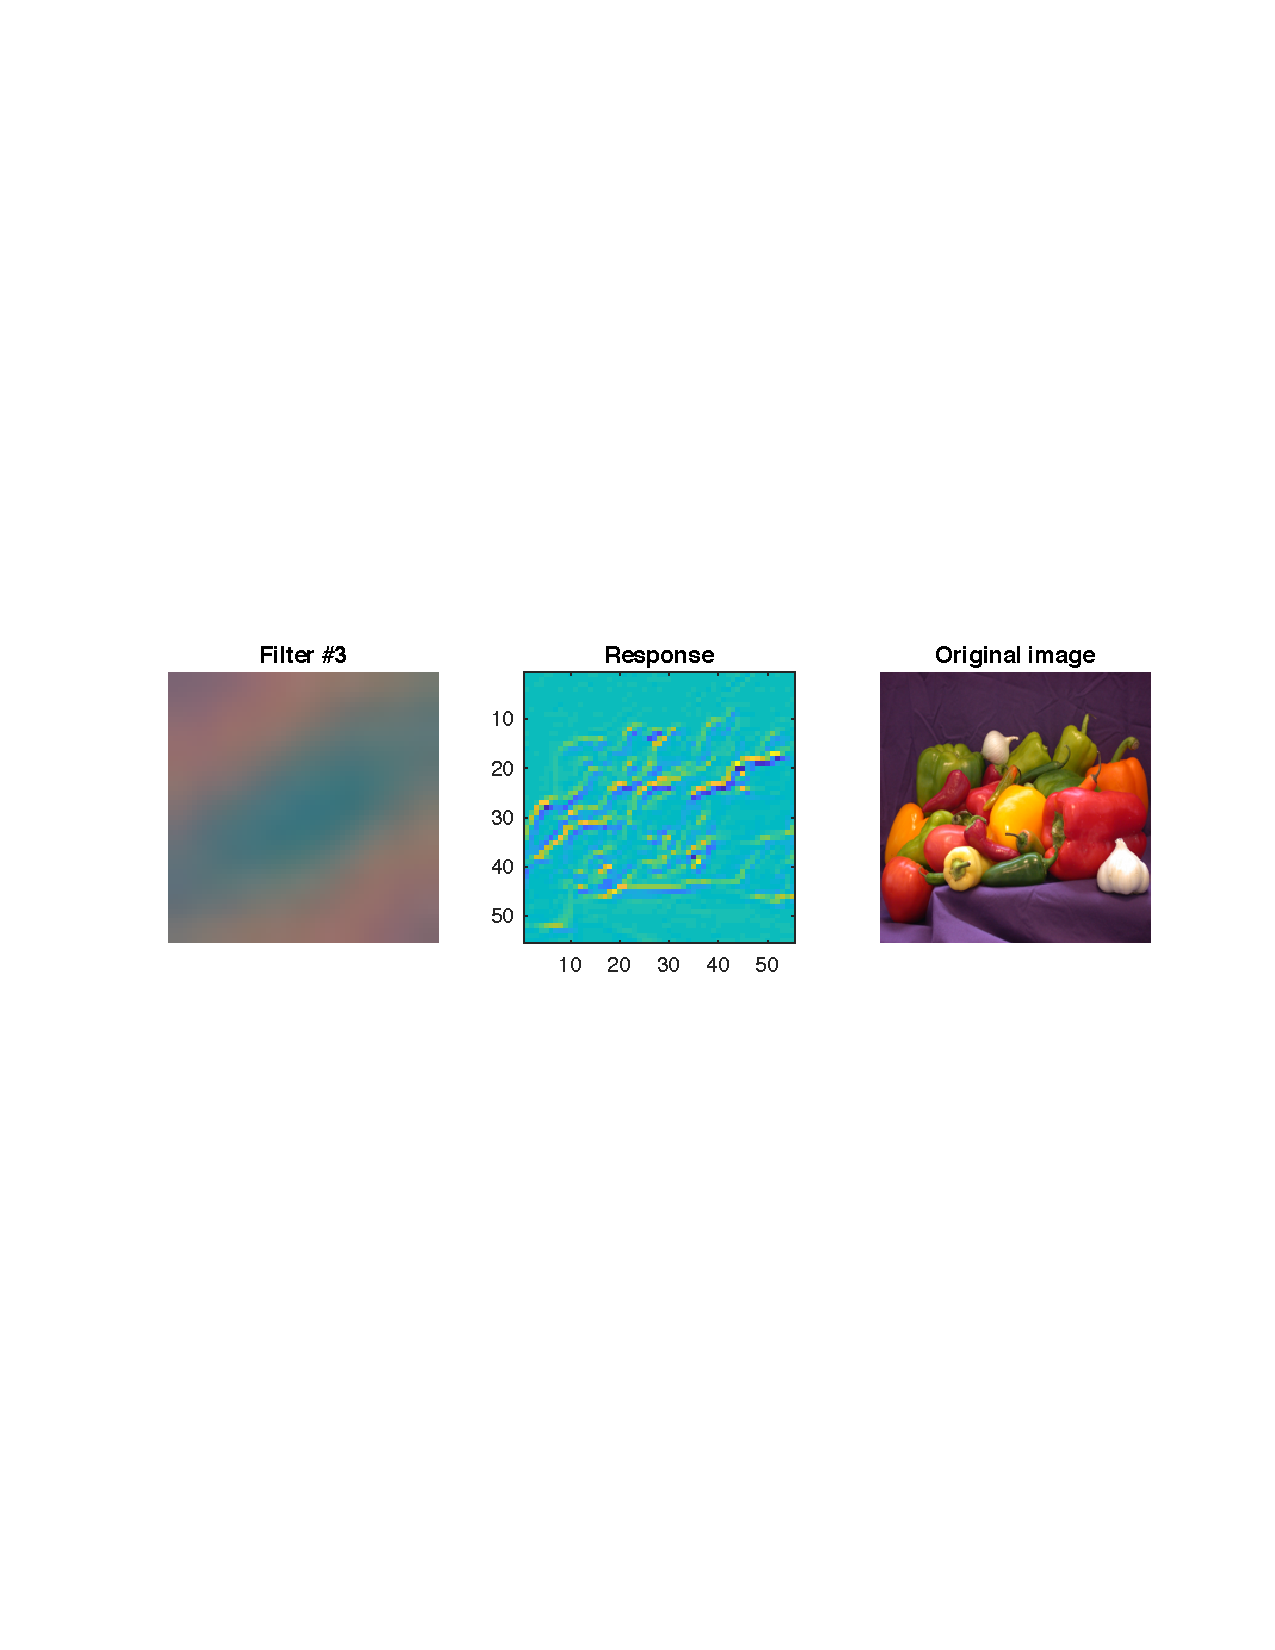
\includegraphics[width=0.7\linewidth]{problem2Bfilter3.pdf}
    \caption{Filter 3 is selective for a diagonal edge in the middle of its receptive field. Specifically, the edge should should consist of a band of higher blue intensity with bands of higher red intensity on either side.}
    \label{fig:my_label}
\end{figure}
\begin{figure}[H]
    \centering
    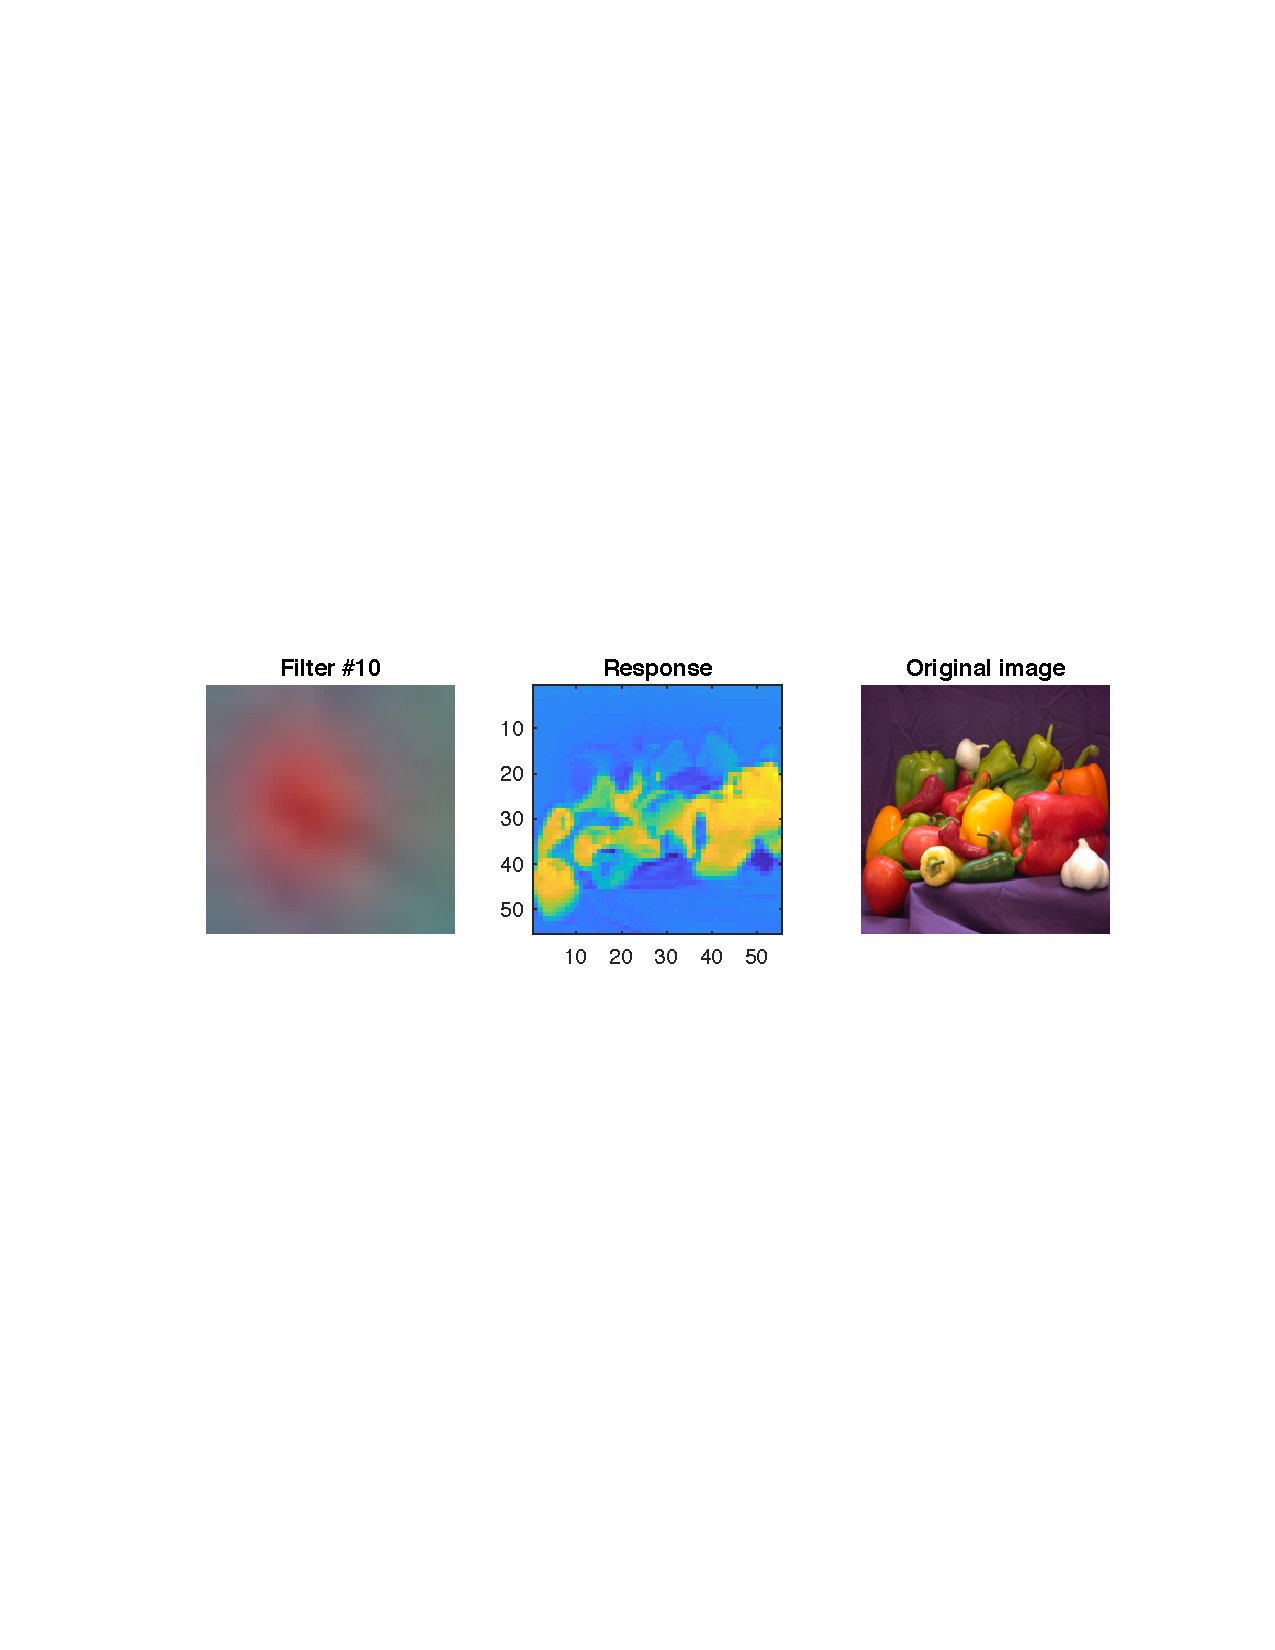
\includegraphics[width=0.7\linewidth]{problem2Bfilter10.pdf}
    \caption{Filter 10 looks like a center-surround neuron sensitive to areas of red surrounded by areas of green. As we can see in the response, this ultimately means that the filter is highly selective for red, orange, and yellow objects.}
    \label{fig:my_label}
\end{figure}
\begin{figure}[H]
    \centering
    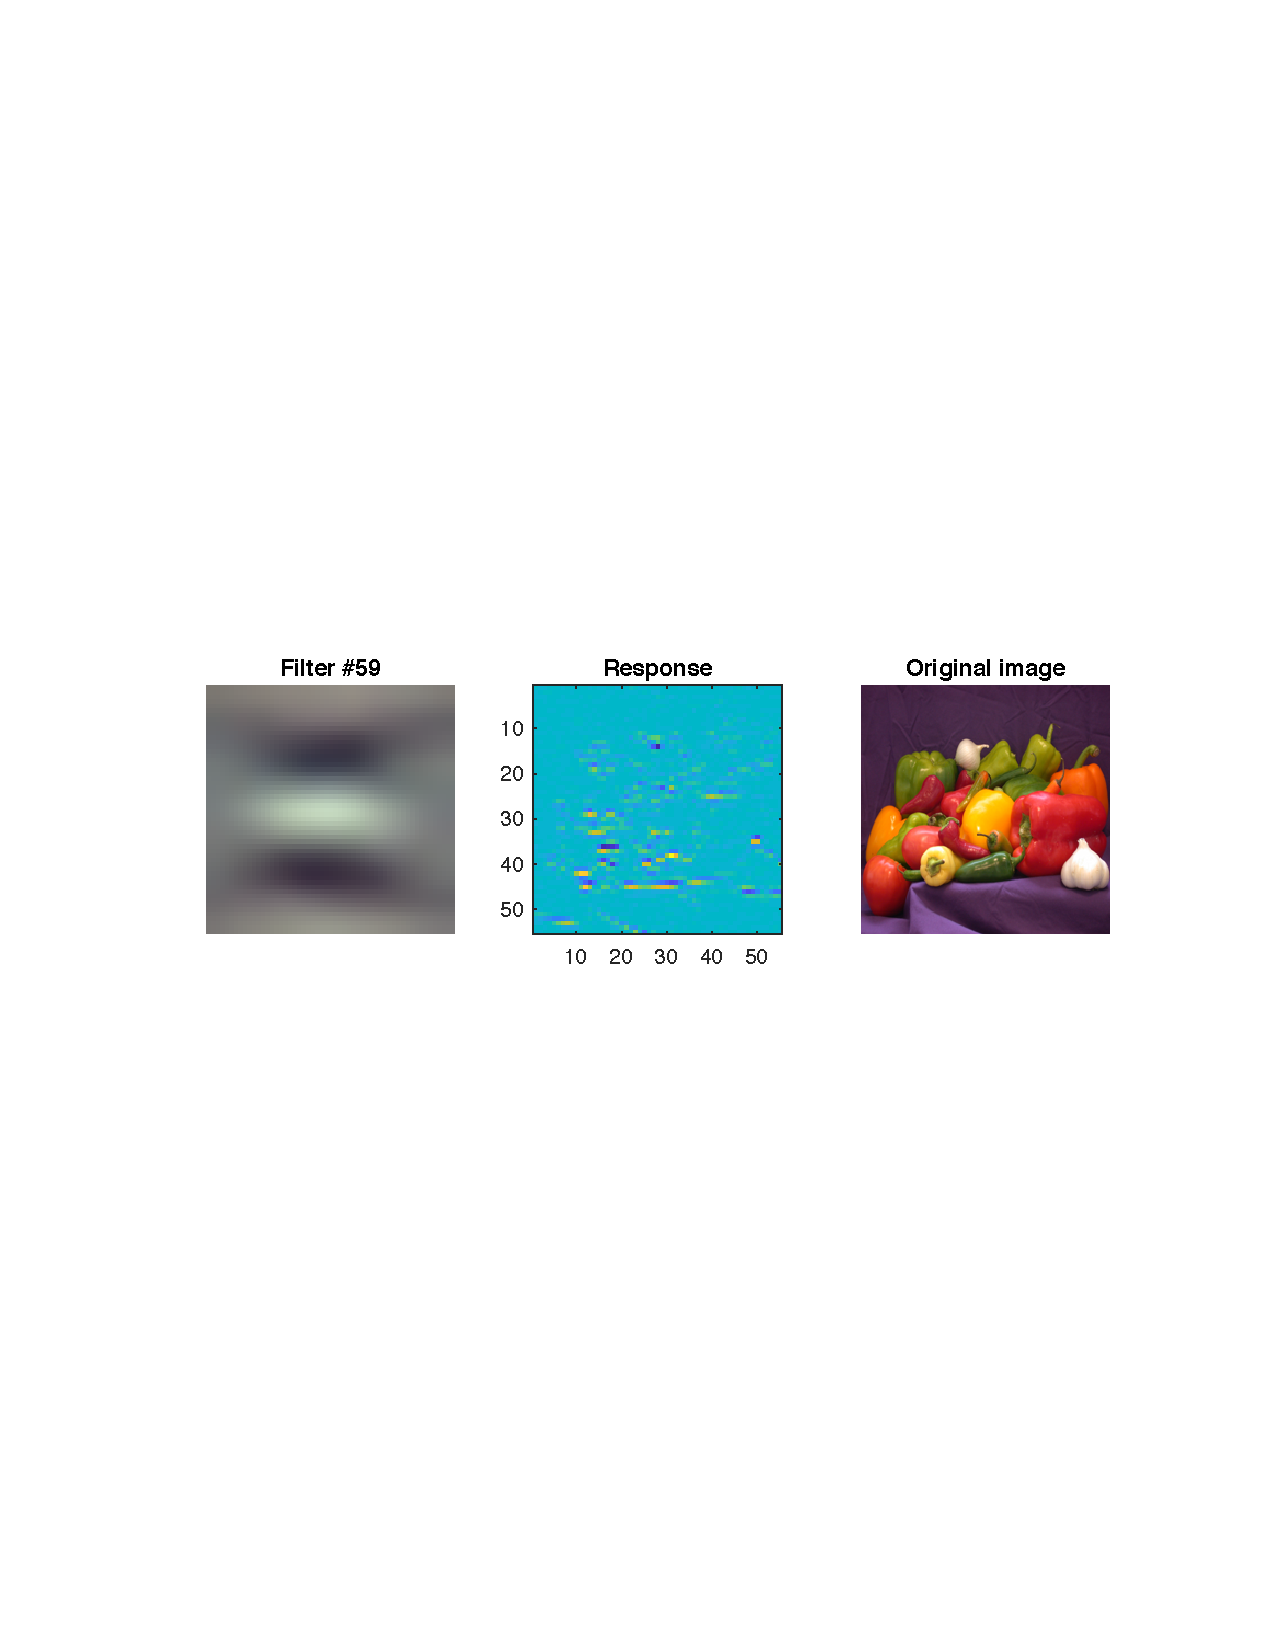
\includegraphics[width=0.7\linewidth]{problem2Bfilter59.pdf}
    \caption{Filter 59 is sensitive to thick, high-contrast, horizontal edges of any color directly in the middle of its receptive field. }
    \label{fig:my_label}
\end{figure}

\subsection*{2c}
\begin{figure}[H]
    \centering
    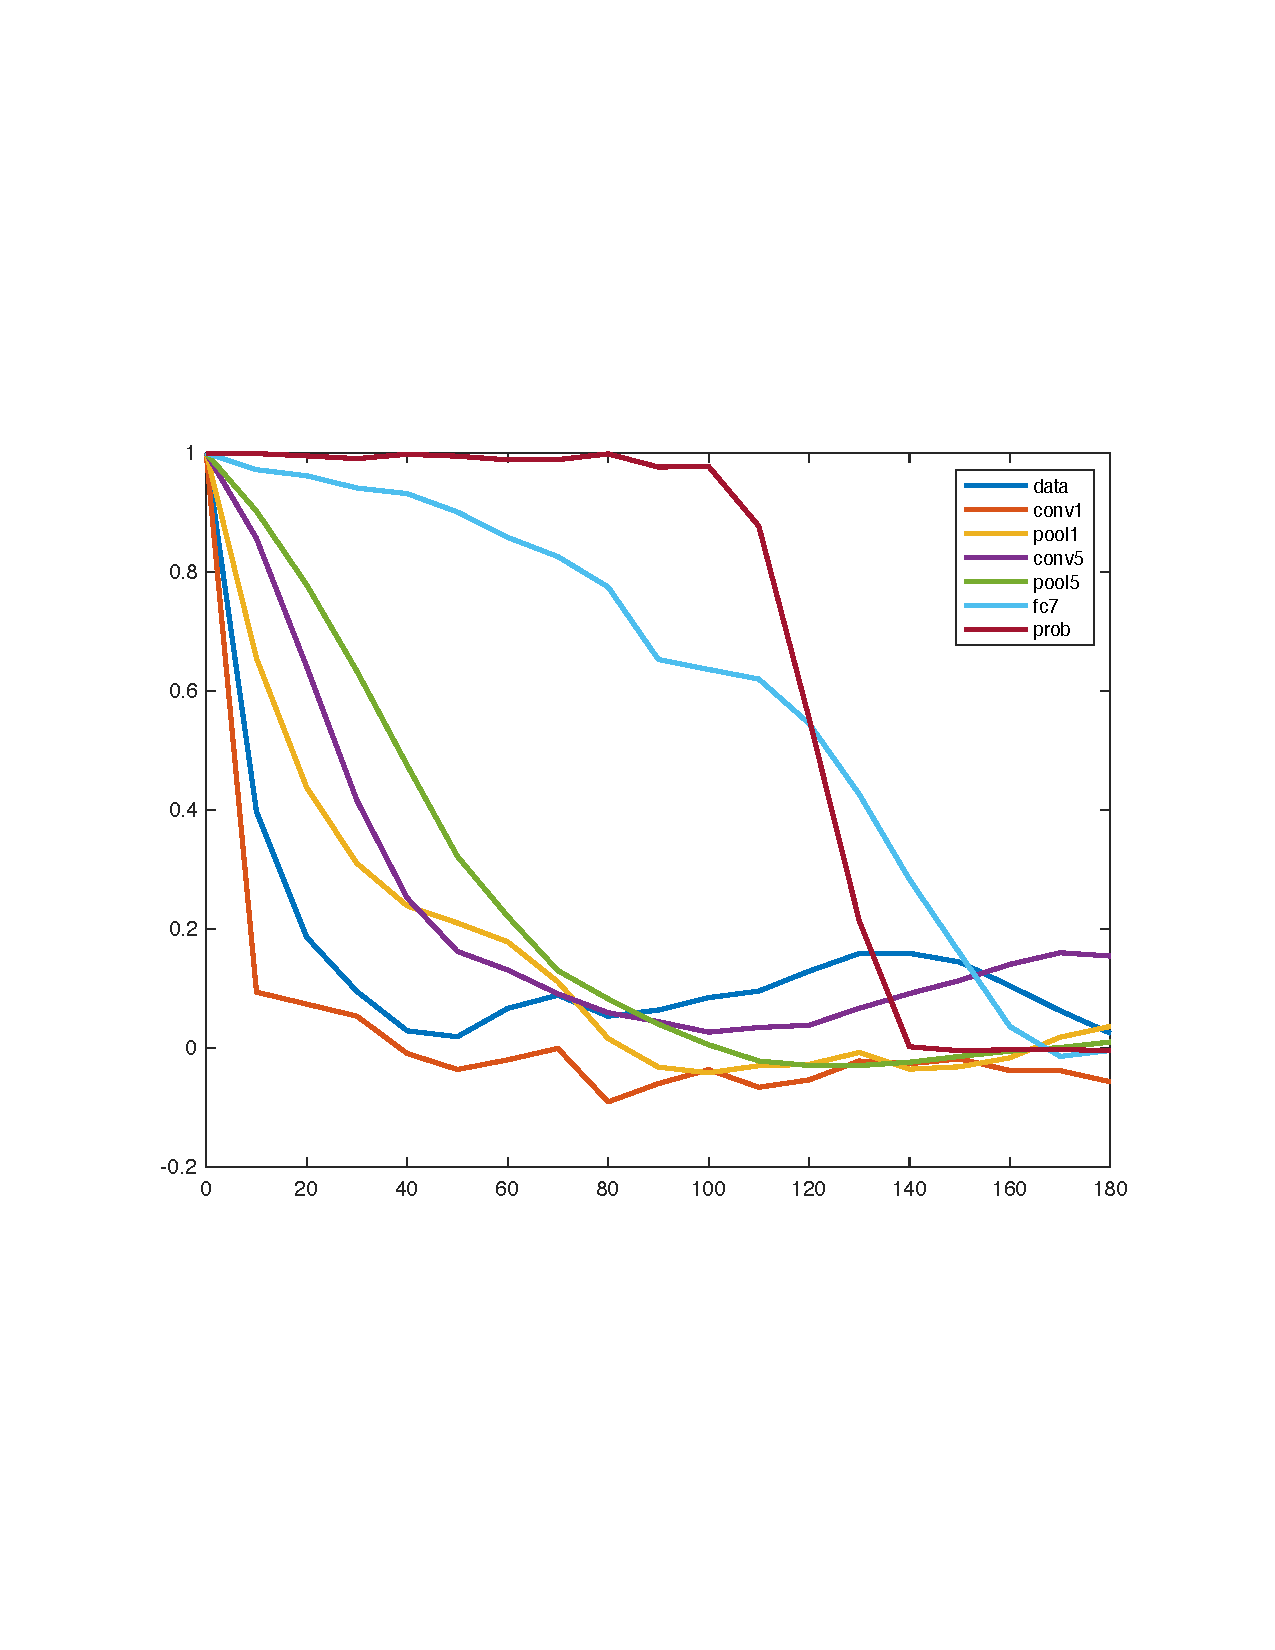
\includegraphics[width=0.7\linewidth]{problem2C.pdf}
    \caption{From this plot, it is evident that higher layers exhibit more translation invariance, where a higher correlation indicates a higher degree of invariance. The output of \texttt{prob} essentially does not begin to change until around 100 pixels of translation. Additionally, the output of \texttt{fc7} changes far more slowly than the lower layers with respect to translation, and the correlation for \texttt{conv5} and \texttt{pool5} are both consistently at least as high the correlation for \texttt{conv1} and \texttt{pool1}. We also observe that \texttt{pool1} is far more robust to translation than \texttt{conv1}, and \texttt{pool5} is initially more invariant than \texttt{conv5}. The fact that, at least at lower amounts of translation, the pooling layers exhibit more invariance than the convolution layers makes sense, given that the pooling operation itself has a certain amount of invariance built into it.}
    \label{fig:my_label}
\end{figure}

\subsection*{2d}
\begin{figure}[H]
    \centering
    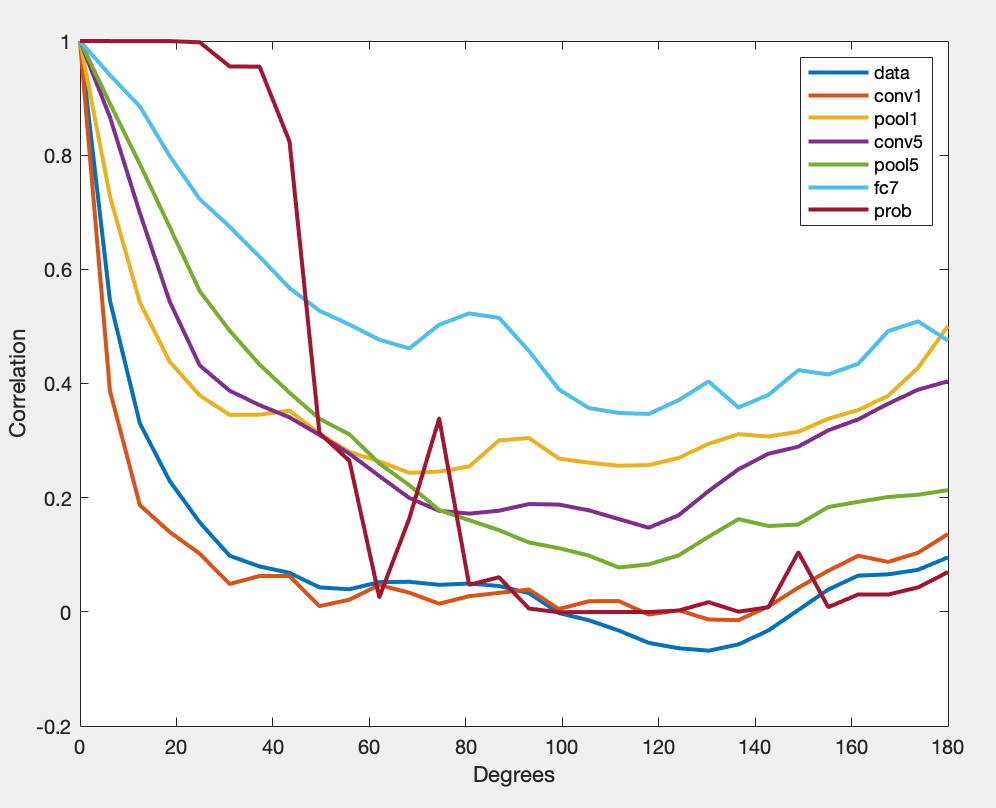
\includegraphics[width=0.7\linewidth]{problem2D_2.png}
    \caption{The correlation for most layers reduced to less than 0.5 within 40-50 degrees, so AlexNet seems to begin to misclassify at around 50 degrees of rotation. While the \texttt{prob} layer showed higher invariance to translation than rotation, the rest of the layers seem generally more invariant to rotation. The correlations dipped below 0.2 for most layers within 60 pixels of translation, while the rotation correlations have a wider distribution between 0 and 0.5, so it seems that AlexNet is more resistant to rotation.}
    \label{fig:my_label}
\end{figure}

\subsection*{2e}
\begin{figure}[H]
    \centering
    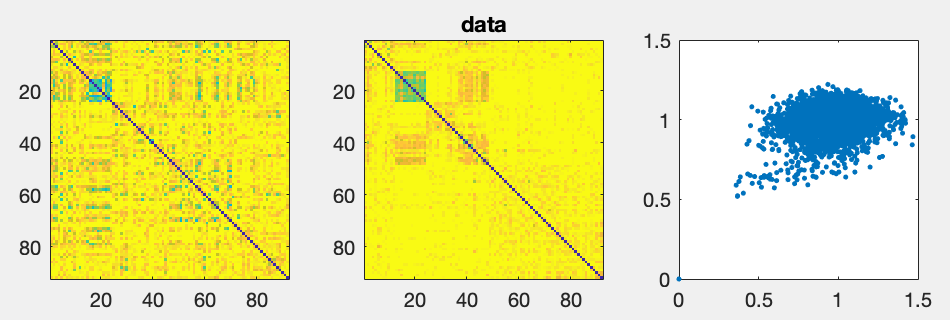
\includegraphics[width=0.7\linewidth]{problem2E_RDMdata.png}
    \label{fig:my_label}
\end{figure}

\begin{figure}[H]
    \centering
    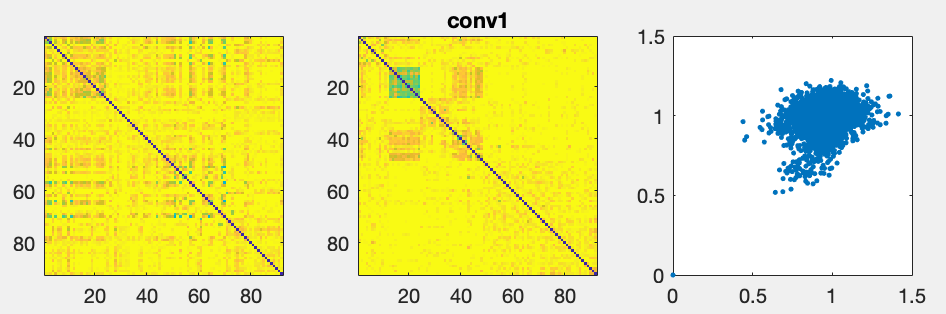
\includegraphics[width=0.7\linewidth]{problem2E_RDMconv1.png}
    \label{fig:my_label}
\end{figure}

\begin{figure}[H]
    \centering
    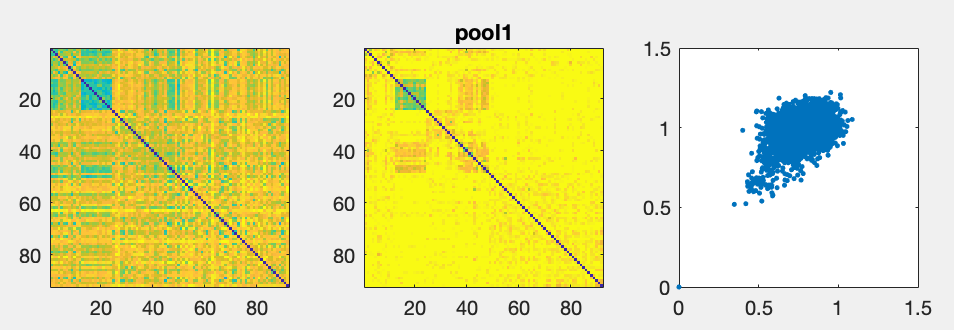
\includegraphics[width=0.7\linewidth]{problem2E_RDMpool1.png}
    \label{fig:my_label}
\end{figure}

\begin{figure}[H]
    \centering
    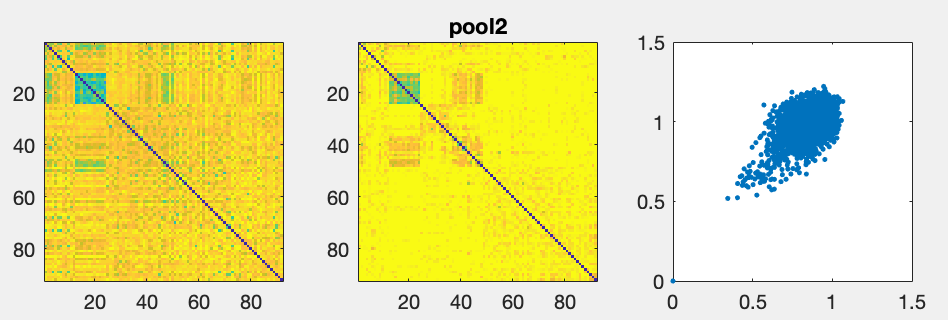
\includegraphics[width=0.7\linewidth]{problem2E_RDMpool2.png}
    \label{fig:my_label}
\end{figure}

\begin{figure}[H]
    \centering
    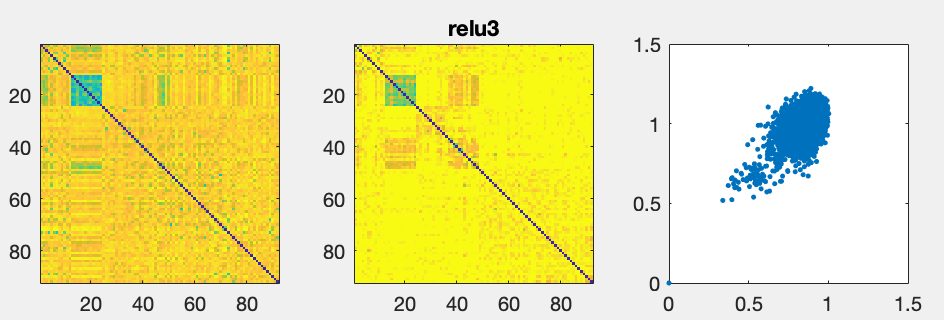
\includegraphics[width=0.7\linewidth]{problem2E_RDMrelu3.png}
    \label{fig:my_label}
\end{figure}

\begin{figure}[H]
    \centering
    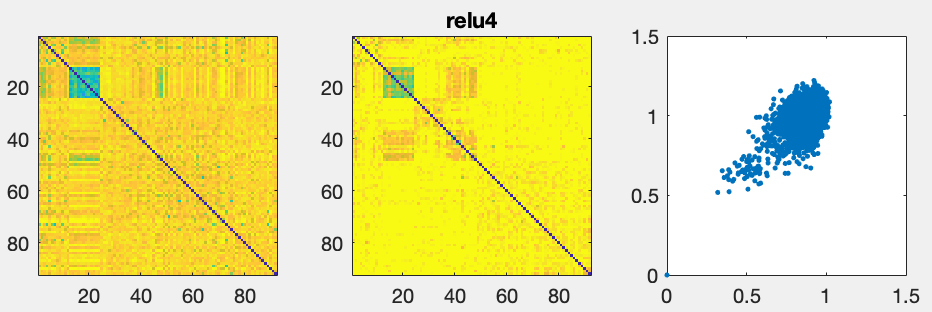
\includegraphics[width=0.7\linewidth]{problem2E_RDMrelu4.png}
    \label{fig:my_label}
\end{figure}

\begin{figure}[H]
    \centering
    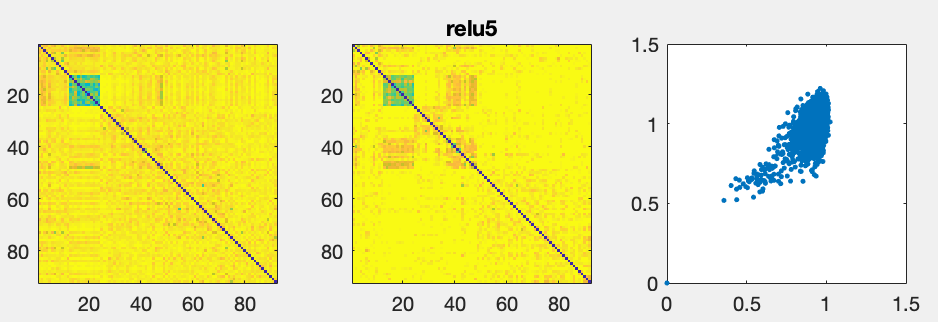
\includegraphics[width=0.7\linewidth]{problem2E_RDMrelu5.png}
    \label{fig:my_label}
\end{figure}

\begin{figure}[H]
    \centering
    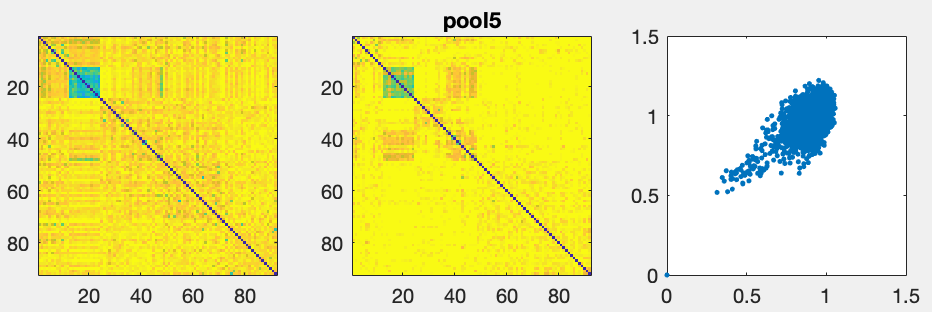
\includegraphics[width=0.7\linewidth]{problem2E_RDMpool5.png}
    \label{fig:my_label}
\end{figure}

\begin{figure}[H]
    \centering
    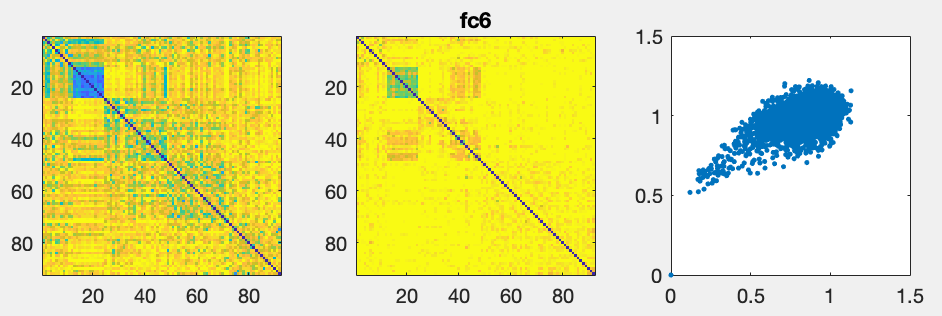
\includegraphics[width=0.7\linewidth]{problem2E_RDMfc6.png}
    \label{fig:my_label}
\end{figure}

\begin{figure}[H]
    \centering
    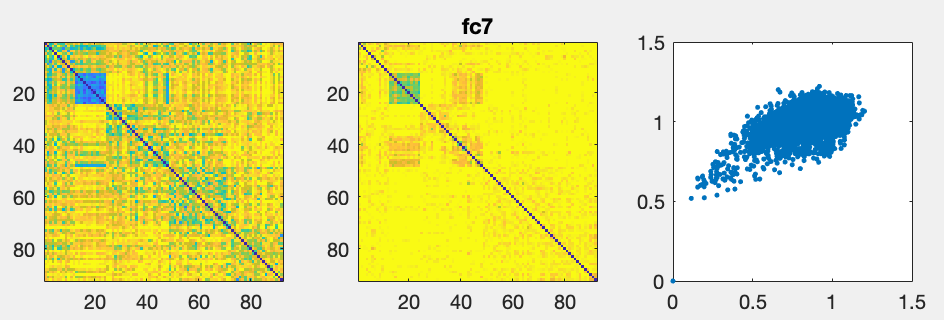
\includegraphics[width=0.7\linewidth]{problem2E_RDMfc7.png}
    \label{fig:my_label}
\end{figure}

\begin{figure}[H]
    \centering
    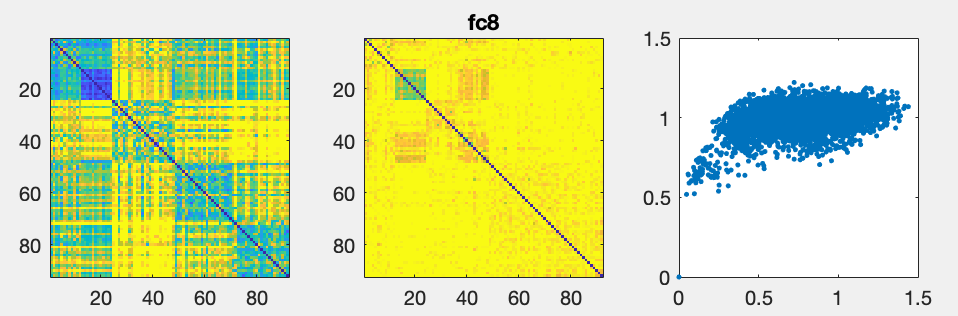
\includegraphics[width=0.7\linewidth]{problem2E_RDMfc8.png}
    \label{fig:my_label}
\end{figure}

\begin{figure}[H]
    \centering
    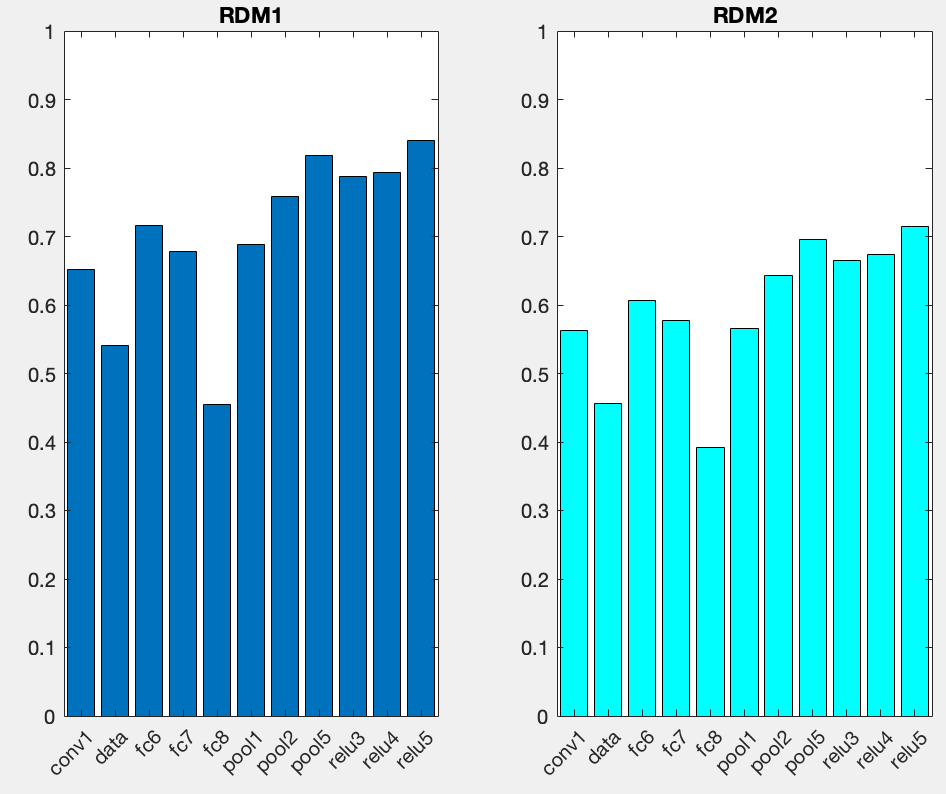
\includegraphics[width=0.7\linewidth]{problem2E_RDMcorrelations.png}
    \label{fig:my_label}
    \caption{The RDMs in intermediate layers of AlexNet are generally more similar to the experimental RDMs than the raw data. The layer of AlexNet that best matches the experimental RDMS is the relu5 layer, followed closely by pool5.}
\end{figure}

\section*{Problem 3}
\subsection*{3a}
\begin{figure}[H]
    \centering
    \includegraphics[width=0.7\linewidth]{problem3A_2.png}
    \label{fig:my_label}
\end{figure}

\subsection*{3b}
The accuracy stayed around 0.5 for the first 1500 iterations, before suddenly spiking to 0.95 and gradually increasing for subsequent iterations. There may be minimal overfitting since a positive difference between the accuracy of the training and test data develops after 2000 trials. The test accuracy doesn't seem to decrease after a certain iteration, so it doesn't seem like stopping earlier would help the accuracy.

\subsection*{3c}
\begin{figure}[H]
    \centering
    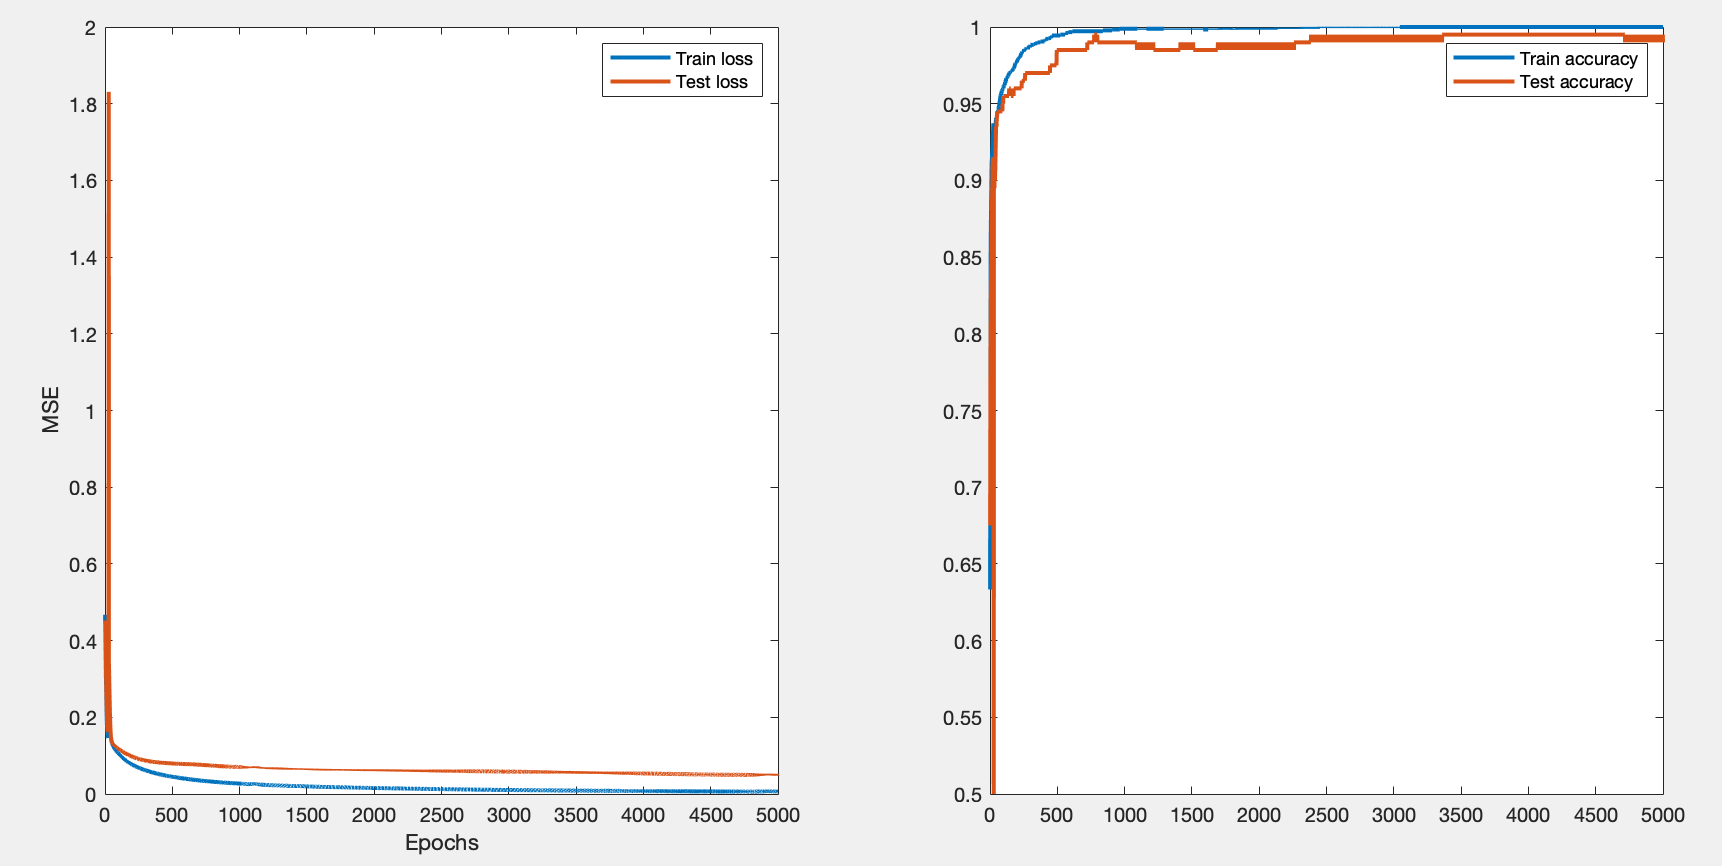
\includegraphics[width=0.7\linewidth]{problem3C.png}
    \caption{The accuracy now spikes towards 1 far more quickly and the final accuracy is closer to 1. Stopping early would not significantly improve the accuracy, since it hovers at the same level after the 2500th iteration. Based on this, a larger weight variance seems better for the purpose of generalization.}
    \label{fig:my_label}
\end{figure}

\end{document}
